\documentclass[UTF8]{ctexart}
\usepackage{amsmath}
\usepackage{mathtools}
\usepackage{geometry}
\usepackage{tikz}
\usepackage{enumitem}
\setitemize{topsep=-0.3cm}
\geometry{a4paper,scale=0.75}
\title{每日一题(3.2)答案}
\author{选题人:王一丁,李政毅\\答案制作:程昊一}
\begin{document}
\maketitle
\begin{enumerate}
\item {\large\CJKfamily{kai}求所有这样的素数,它加上10或14后,仍为素数.}\\
\hspace*{2em}\textbf{解}\quad 设这个素数为$p$.现对$p$除以3的余数进行分类讨论.\\
\begin{itemize}
\item[(1)] 若$p$除以3的余数为1,则$3|(p+14)$,而$3<p+14$,所以$p+14$不是素数,与题设矛盾.\\
\item[(2)] 若$p$除以3的余数为2,则$3|(p+10)$,而$3<p+10$,所以$p+10$不是素数,与题设矛盾.\\
\item[(3)] 若$p$除以3的余数为0,即$p$是3的倍数,又$p$为素数,所以$p=3$.此时$p+10=13,p+14=17$,均为素数,成立.\\
\end{itemize}
\hspace*{2em}综上:有且仅有一个素数3满足要求.
\item {\large\CJKfamily{kai}证明:从1至100(包括1和100)中任选51个数,其中必有两个数互素.\\
思考:题中的“51”还可以更小吗?}\\
\hspace*{2em}\textbf{分析}\quad 在某些元素中任取一部分元素,这使我们联想到抽屉原理.\\
\hspace*{2em}\textbf{解}\quad 构造抽屉:
\[\{1,2\},\{3,4\},\{5,6\}\dots\{99,100\}\]
(表示1和2为一个抽屉,3和4为一个抽屉,等等.)\\
\hspace*{2em}共计50个抽屉.因为有51个数,所以必然存在两个数,它们在同一个抽屉中,那么此两数相邻,所以它们互素.\\
\hspace*{2em}综上:必然存在两个互素的数.\\
\hspace*{2em}题中的“51”并不能更小.事实上,若取的数小于51个,那么我们可以全部取偶数,这样每个数的最大公因数至少为2,命题不成立.\\
\item {\large\CJKfamily{kai}将平面上所有的点都染成红、蓝两色,证明:存在一条长为1的线段,它的端点同色.\\
思考:若平面不为全红或全蓝,是否总存在一条长为1的线段,其端点异色?若将平面染成三种颜色,是否仍然存在长为1的端点同色的线段?}\\
\hspace*{2em}\textbf{解}\quad 在已染色的平面内任取一个边长为1的等边三角形.则这个三角形的三个顶点均可能为红、蓝两色.由抽屉原理可知(在此处苹果为点,抽屉为两种颜色,即“染色类”),必有两个顶点同色.这时,此两顶点的距离为1,存在性得证.\\
\\
\hspace*{2em}下面为“思考”部分的解答,较难,没有兴趣的同学可以跳过.\\
\hspace*{2em}事实上,长为1的、端点异色的线段是存在的.我们分以下两部分证明.\\
\begin{itemize}
\item[(1)]{\large\CJKfamily{fs}存在一个长度不大于2的、端点异色的线段.}\\
\hspace*{2em}因为平面并不是全红或全蓝,所以必然存在两个异色的点,设为$A$和$B$.连接$AB$.不妨设$A$为红色,$B$为蓝色.\\
\hspace*{2em}若$AB\le2$,则命题成立.\\
\hspace*{2em}若$AB>2$,我们使用反证法.假设不存在长度不大于2的、端点异色的线段,那么在$AB$上截取点$A_1$使得$AA_1=2$.由于我们的假设,$A_1$与$A$同色,均为红色.\\
\hspace*{2em}在$A_1B$上截取点$A_2$,使得$A_1A_2=2$.由于我们的假设,$A_2$与$A_1$同色,均为红色.\\
\hspace*{2em}在$A_2B$上截取点$A_3$,使得$A_2A_3=2$.由于我们的假设,$A_3$与$A_2$同色,均为红色.\\
\hspace*{2em}这样一直截取下去到$A_n$,使得$A_nB\le2$,这时$A_n$与$A$同色,均为红色,此时$A_n$与$B$异色,且\\$A_nB\le2$,与假设矛盾.\\
\hspace*{2em}所以,假设不成立,原命题成立.\\
\begin{figure}[!ht]
\centering
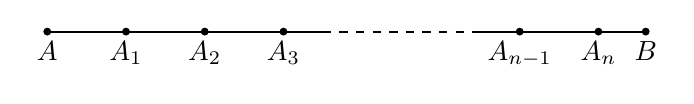
\begin{tikzpicture}
	\node at(0,0) [anchor=north]{$A$};
	\node at(1,0) [anchor=north]{$A_1$};
	\node at(2,0) [anchor=north]{$A_2$};
	\node at(3,0) [anchor=north]{$A_3$};
	\node at(6,0) [anchor=north]{$A_{n-1}$};
	\node at(7,0) [anchor=north]{$A_n$};
	\node at(7.6,0) [anchor=north]{$B$};
	\foreach \x in{0,1,2,3,6,7,7.6}
		\fill (\x,0) circle(0.05);
	\draw [thick](0,0)--(3.5,0);
	\draw [thick,dashed](3.5,0)--(5.5,0);
	\draw [thick](5.5,0)--(7.6,0);
\end{tikzpicture}
\end{figure}
\item[(2)]{\large\CJKfamily{fs}存在一条长为1的、端点异色的线段}\\
\hspace*{2em}假设我们有一条长度不大于2的、端点异色的线段,设为线段$AB$.在(1)中,我们已经证明了线段$AB$的存在性.现在,分别以$A$和$B$为圆心,1为半径画圆,两圆交于$P,Q$两点.\\
\hspace*{2em}现在我们研究点$P$的颜色.事实上,由于$A,B$是异色的,所以无论$P$是什么颜色,$A,B$中都有与之异色的点,这时便存在一条长为1且端点异色的线段.\\

\begin{figure}[!ht]
\centering
\begin{tikzpicture}
	\fill (0,0) circle(0.05);
	\fill (4,0) circle(0.05);
	\draw (0,0) circle(2.5);
	\draw (4,0) circle(2.5);
	\fill (2,1.5) circle(0.05);
	\fill (2,-1.5) circle(0.05);
	\node at(0,0)[anchor=east]{$A$};
	\node at(4,0)[anchor=west]{$B$};
	\node at(2,1.5)[anchor=south]{$P$};
	\node at(2,-1.5)[anchor=north]{$Q$};
	\node at(2,-3)[anchor=north]{\CJKfamily{kai}“思考”第一问图};
	\draw [thick](0,0)--(4,0);
	\draw [thick,dashed](0,0)--(2,1.5);
	\draw [thick,dashed](4,0)--(2,1.5);
\end{tikzpicture}
\end{figure}

\end{itemize}
\hspace*{2em}至此,命题得证.\\
\\
对于“思考”的第二问,答案是:存在.下面给出证明:\\
\hspace*{2em}若平面内只有一种颜色,命题显然成立.若平面内只有两种颜色,本题的第一部分已经证明.下面我们考虑三种颜色都用上的情况\\
\hspace*{2em}设三种颜色为红、黄、蓝.分以下两种情况讨论:\\

\begin{itemize}
\item[(1)]若平面内存在长度为$\sqrt{3}$且端点异色的线段,记为$A,B$.不妨设$A$为红色,$B$为蓝色.连接$AB$.分别以$A,B$为圆心,1为半径作圆,设两圆相交与$P,Q$.\\
\hspace*{2em}若$P,Q$中有一个为红色或黄色,则存在一条满足要求的线段,命题成立;若$P,Q$均不为红色或黄色,即$P,Q$均为蓝色.易证$PQ=1$(我们默认能读到这里的人都可以证明).此时$PQ$\\即为长为1且端点同色的线段,命题得证.\\
\hspace*{2em}综上,在这种情况下,无论怎样命题均成立.
\item[(2)]若平面内不存在长为$\sqrt{3}$且端点同色的线段,即每一条长度为$\sqrt{3}$的线段,它的端点均同色.那么,任取一点,以此为圆心,$\sqrt{3}$为半径作圆$c_1$.\\
\hspace*{2em}那么,圆$c_1$上的所有点均同色.在圆上任取一点$C$,以$C$为圆心,1为半径作圆$c_2$,交圆$c_1$于$M$,\\$N$两点.因为$C,M$都在圆$c_1$上,所以$C,M$同色,又$CM=1$,所以$CM$为符合要求的线段,命题成立.
\end{itemize}
\quad\\
\hspace*{2em}综上:命题得证.
\begin{figure}[!ht]
\centering
\begin{tikzpicture}
	\node at(0,0.5)[anchor=east]{$A$};
	\node at(3.46,0.5)[anchor=west]{$B$};
	\node at(1.73,1.5)[anchor=south]{$P$};
	\node at(1.73,-0.5)[anchor=north]{$Q$};
	\fill (0,0.5) circle(0.05);
	\fill (3.46,0.5) circle(0.05);
	\fill (1.73,1.5) circle(0.05);
	\fill (1.73,-0.5) circle(0.05);
	\draw [thick](0,0.5)--(3.46,0.5);
	\draw [thick,dashed](0,0.5)--(1.73,1.5);
	\draw [thick,dashed](0,0.5)--(1.73,-0.5);
	\draw [thick,dashed](3.46,0.5)--(1.73,1.5);
	\draw [thick,dashed](3.46,0.5)--(1.73,-0.5);
	\draw (0,0.5) circle(2);
	\draw (3.46,0.5) circle(2);
	\fill (10,0) circle(0.05);
	\node at(13.03,1.66)[anchor=east]{$c_1$};
	\node at(10,3.46)[anchor=north west]{$C$};
	\draw (10,0) circle(3.46);
	\draw (10,3.46) circle(2);
	\node at(8.09,2.88)[anchor=east]{$M$};
	\node at(11.91,2.88)[anchor=west]{$N$};
	\fill (8.09,2.88) circle(0.05);
	\fill (11.91,2.88) circle(0.05);
	\fill (10,3.46) circle(0.05);
	\draw [thick,dashed](8.09,2.88)--(10,3.46);
	\node at(8.07,3.98)[anchor=east]{$c_2$};
	\node at(1.73,-4)[anchor=north]{\CJKfamily{kai}“思考”第二问(1)图};
	\node at(10,-4)[anchor=north]{\CJKfamily{kai}“思考”第二问(2)图};

\end{tikzpicture}
\end{figure}

\end{enumerate}

\end{document}